\documentclass[11pt]{article}
\usepackage[margin=0.66in]{geometry}
\usepackage{booktabs,enumitem,fancyhdr,graphicx,tabularx,titlesec}
\usepackage[table]{xcolor}
\usepackage[hidelinks]{hyperref}
\graphicspath{{docs/lessons/assets/}{../assets/}}
\hypersetup{pdftitle={ADK Lesson 044: Board-Frame Orientation and Presentation Intent},
 pdfauthor={Kevin Shanahan},
 pdfsubject={Synthetic gravity orientation and bounded light and tone intent},
 pdflang={en-US}}
\pagestyle{fancy}\fancyhf{}
\lhead{\textsc{ADK Lesson 044}}\rhead{Orientation and Presentation Intent}
\cfoot{\thepage}\setlength{\headheight}{14pt}
\setlength{\parindent}{0pt}\setlength{\parskip}{4pt}
\setlist{nosep,leftmargin=1.45em}
\titleformat{\section}{\Large\bfseries}{\thesection}{0.5em}{}
\newcommand{\lessonbox}[1]{\begin{center}\fbox{\parbox{0.92\linewidth}{#1}}\end{center}}
\newcommand{\blankline}{\rule{0.86in}{0.4pt}}

\begin{document}
\begin{center}
 {\Huge\bfseries Board-Frame Orientation}\\[3pt]
 {\Large Turn copied gravity into bounded presentation intent}\\[7pt]
 \fbox{\textbf{E0 SYNTHETIC REPLAY --- NO POWERED INERTIAL MODULE CLAIM}}
\end{center}
\begin{tabularx}{\linewidth}{@{}>{\bfseries}l X >{\bfseries}l X@{}}
Lesson & 044 --- component & Time & 90--120 minutes\\
Prerequisite & Lesson 043 copied observations & Board & compile-only Mega replay\\
Evidence & named memory result cells & Boundary & no bus, pins, wiring, or sensor\\
\end{tabularx}

\lessonbox{\textbf{Responsibility.} Map one current, nonsaturated copied
observation into gravity-relative pitch and roll, then map that estimate into
light and tone \emph{intent}. The policies own no endpoint or clock. They do
not estimate yaw, heading, position, velocity, gestures, or navigation.}

\section{Name the board frame}
\begin{center}
% ADK visual: pencil
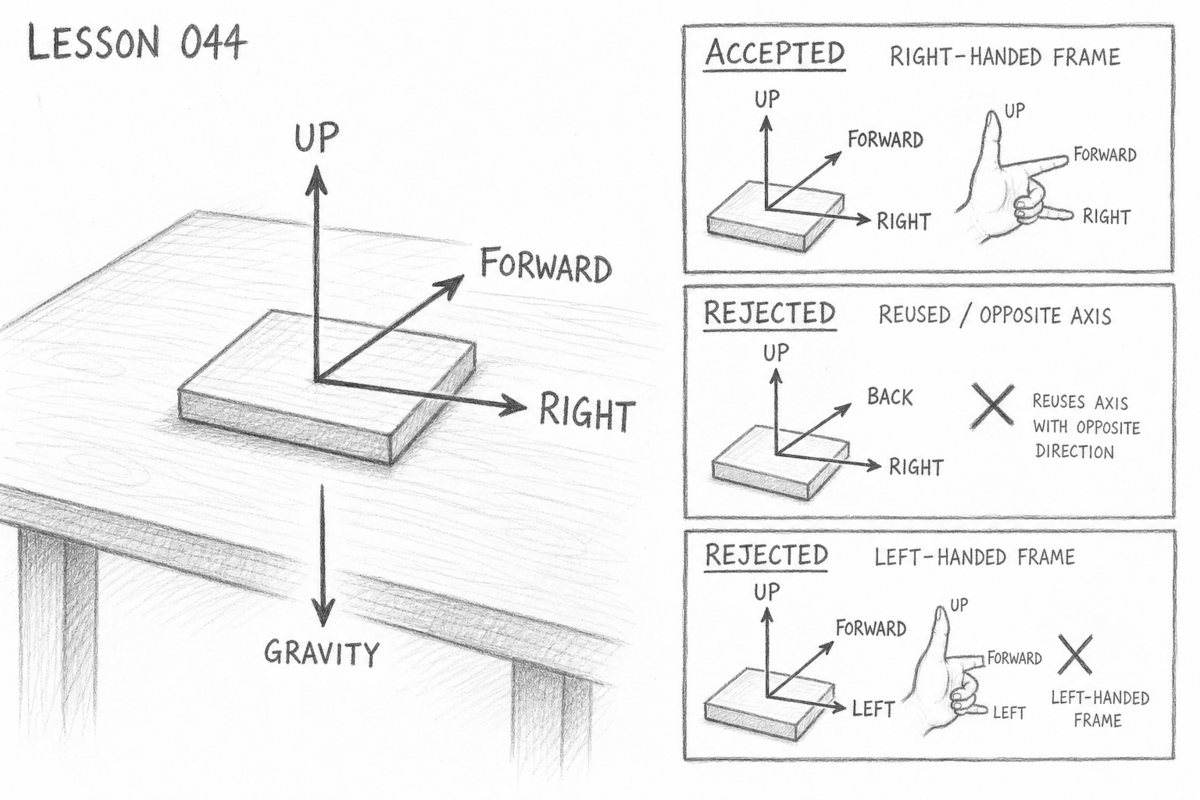
\includegraphics[width=0.96\linewidth,height=0.29\textheight,
 keepaspectratio]{044-board-frame-gravity-pencil.png}

\small\textit{Alternative text: a pencil drawing labels right, forward, and up
on a stationary tabletop board, then shows gravity resolved into those three
axes for pitch and roll.}
\end{center}

Mounting is configuration, not an assumption. Choose three distinct signed
sensor axes for board right \(R\), forward \(F\), and up \(U\). They must form
a right-handed frame. Duplicate axes, opposite reuse of one axis, and
left-handed frames are rejected during initialization.

\begin{tabularx}{\linewidth}{@{}l X X@{}}
\toprule
Board direction & Signed sensor axis & How you checked right-handedness\\
\midrule
right & \blankline & \blankline\\[8pt]
forward & \blankline & \blankline\\[8pt]
up & \blankline & \blankline\\
\bottomrule
\end{tabularx}

Only a \texttt{Current} Lesson 043 observation with both readiness fields
true, nonzero configuration, calibration, and freshness revisions, nonzero
maximum age, no saturation, and OK status is eligible.
Gravity magnitude outside its configured band or any rate beyond the
stationary threshold yields \texttt{Unsteady}, not a motion estimate.

\newpage
\section{Predict poses before calculating}
\begin{center}
% ADK visual: pencil
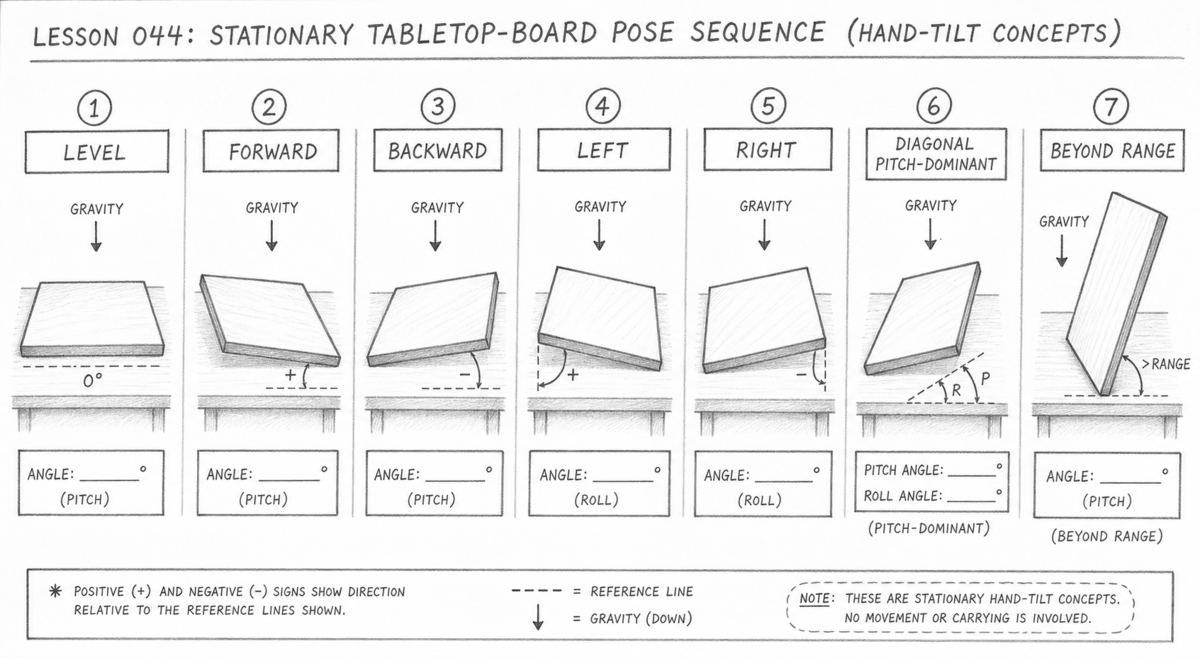
\includegraphics[width=0.97\linewidth,height=0.27\textheight,
 keepaspectratio]{044-orientation-poses-pencil.png}

\small\textit{Alternative text: pencil sketches show a level board, four
cardinal tilts, and a diagonal tilt, with positive pitch pointing forward and
positive roll pointing right.}
\end{center}

For remapped acceleration \(R,F,U\), work in micro-g:
\[
 h=\lfloor\sqrt{R^2+U^2}\rfloor,\qquad
 pitch=\mathrm{atan2}(F,h),\qquad
 roll=\mathrm{atan2}(R,U).
\]
The implementation uses widened integer arithmetic and a normalized 16-step
CORDIC. Its test oracle permits at most 4 millidegrees error. That error is
included conservatively at level and presentation thresholds.

\begin{tabularx}{\linewidth}{@{}l r r r X@{}}
\toprule
Pose & \(R\) (\(\mu g\)) & \(F\) (\(\mu g\)) & \(U\) (\(\mu g\)) & Prediction\\
\midrule
level & \blankline & \blankline & \blankline & \blankline\\[7pt]
forward & \blankline & \blankline & \blankline & \blankline\\[7pt]
right & \blankline & \blankline & \blankline & \blankline\\[7pt]
diagonal & \blankline & \blankline & \blankline & \blankline\\
\bottomrule
\end{tabularx}

\subsection*{Fixed-point worksheet}
\begin{tabularx}{\linewidth}{@{}X X X X@{}}
\toprule
\(h\) (\(\mu g\)) & pitch (mdeg) & roll (mdeg) & quality\\
\midrule
\rule{0pt}{16pt}\blankline & \blankline & \blankline & \blankline\\[9pt]
\blankline & \blankline & \blankline & \blankline\\
\bottomrule
\end{tabularx}

Both absolute angles inside the conservative level bound yield
\texttt{Level}. An angle in a threshold error band stays \texttt{Tilted}; an
angle outside the conservative maximum yields
\texttt{BeyondPresentationRange}. At a diagonal tie, pitch wins: positive
pitch is \texttt{Forward}; negative pitch is \texttt{Backward}. Positive roll
is \texttt{Right}; negative roll is \texttt{Left}.

\newpage
\section{Convert an estimate into intent}
\begin{center}
% ADK visual: pencil
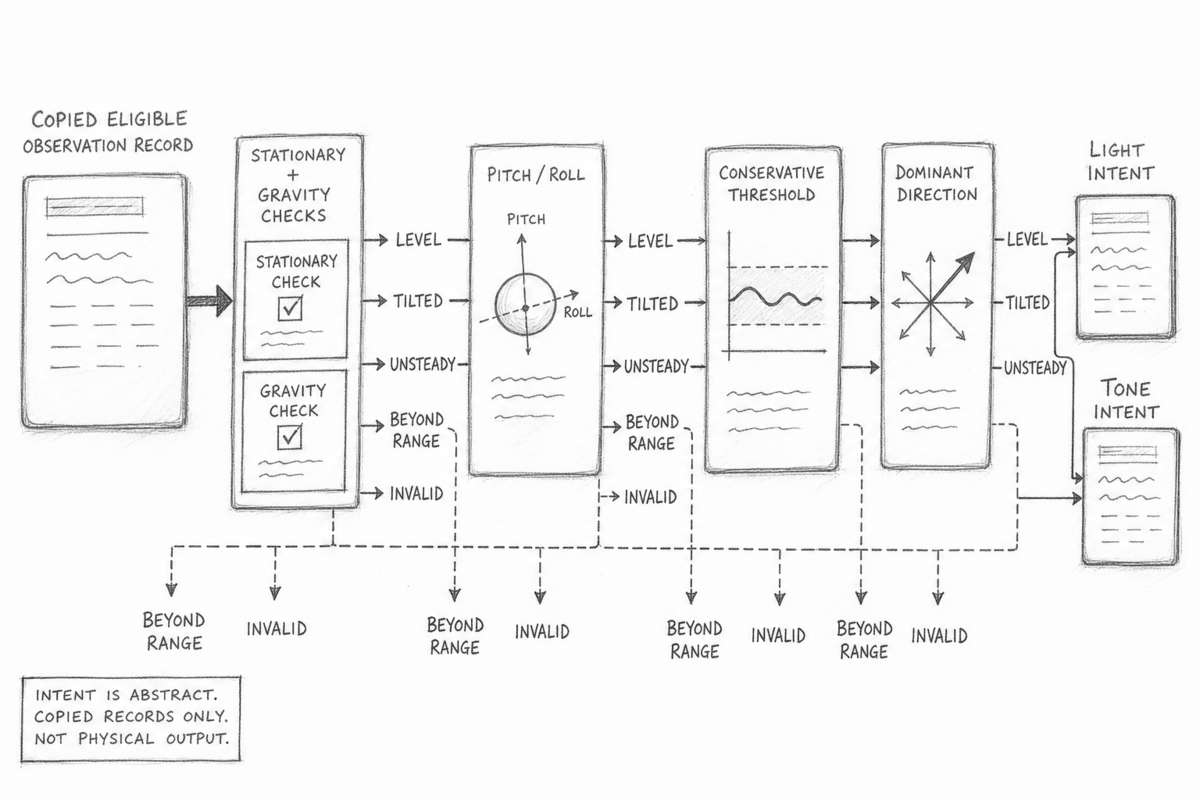
\includegraphics[width=0.96\linewidth,height=0.26\textheight,
 keepaspectratio]{044-presentation-intent-pencil.png}

\small\textit{Alternative text: a pencil flow maps level, four tilt
directions, unsteady, beyond-range, and invalid estimates to complete RGB and
tone intent records without drawing or claiming physical endpoints.}
\end{center}

\begin{tabularx}{\linewidth}{@{}l X X@{}}
\toprule
Quality & Complete light intent & Tone intent\\
\midrule
\texttt{Level} & configured level frame & disabled\\
\texttt{Tilted} & directional frame, scaled and clamped & only on direction change\\
\texttt{Unsteady} & phase A or B supplied by caller & disabled\\
\texttt{BeyondPresentationRange} & configured fault-safe frame & disabled\\
\texttt{Invalid}/non-OK & configured invalid frame & disabled\\
\bottomrule
\end{tabularx}

For a tilted estimate, calculate the unclamped intensity:
\[
 I=\frac{|dominantAngle|\times sensitivityPermille}
          {fullScaleAngleMilliDegrees}.
\]
All angles are millidegrees and sensitivity is 1--1000 permille. The widened
product prevents overflow. Clamp \(I\) to the configured minimum and maximum;
do not wrap it.

\begin{tabularx}{\linewidth}{@{}X X X X@{}}
\toprule
dominant angle (mdeg) & sensitivity (permille) & full scale (mdeg) & intensity (permille)\\
\midrule
\rule{0pt}{16pt}\blankline & \blankline & \blankline & \blankline\\[9pt]
\blankline & \blankline & \blankline & \blankline\\
\bottomrule
\end{tabularx}

A bounded tone is intent, not sound. It is enabled only when a valid tilted
direction changes. Replaying the same direction is silent. The caller supplies
\texttt{diagnosticPhase}; the policy contains no hidden timer and never
toggles an LED.

\newpage
\section{Replay and inspect named result cells}
\begin{center}
% ADK visual: pencil
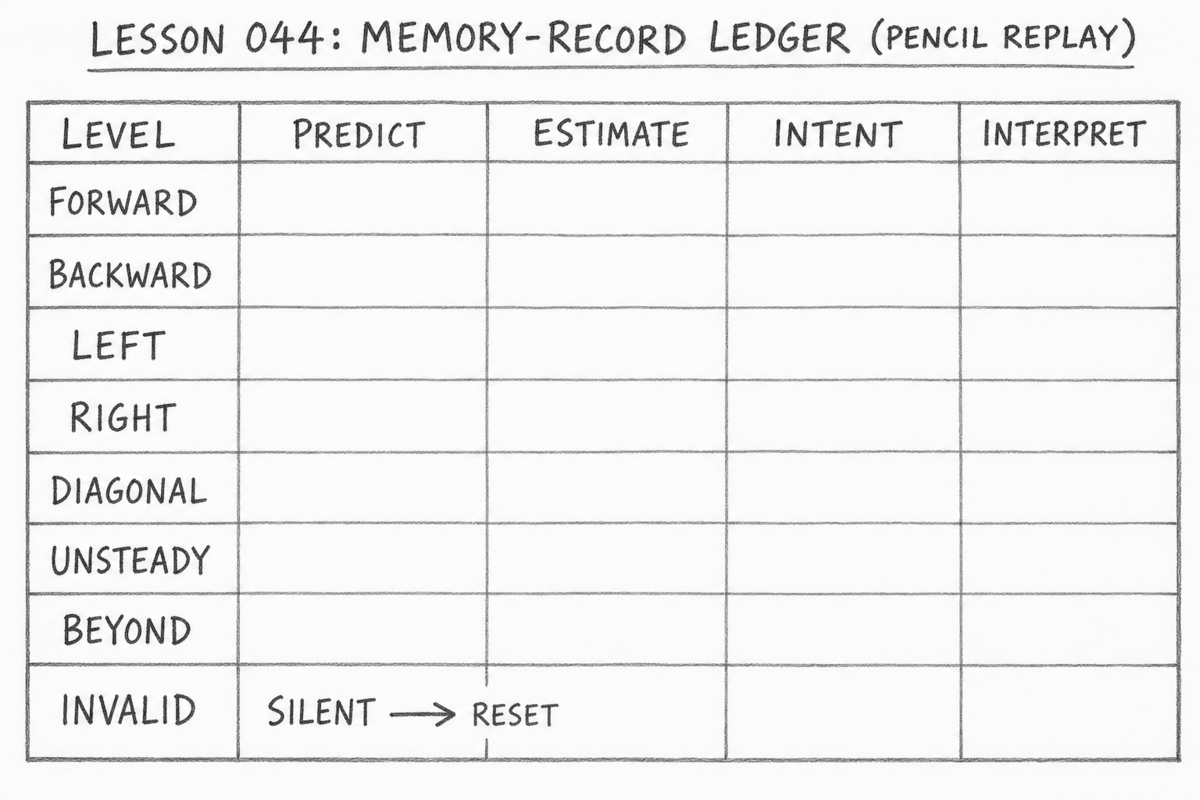
\includegraphics[width=0.95\linewidth,height=0.22\textheight,
 keepaspectratio]{044-replay-worksheet-pencil.png}

\small\textit{Alternative text: a pencil worksheet sends synthetic level,
cardinal, diagonal, unsteady, beyond-range, and invalid frames through
orientation and presentation policies into named memory result cells.}
\end{center}

Use
\href{https://github.com/spincyc/adk/blob/main/examples/Lesson044OrientationPresentation/Lesson044OrientationPresentation.ino}
{the Lesson 044 compile-only replay}. Predict first, then copy the complete
orientation and presentation records. A result cell is host-harness or
simulator evidence; it is not a physical light, sound, or sensor observation.

\begin{tabularx}{\linewidth}{@{}l X X X@{}}
\toprule
Frame & Orientation prediction & Intent prediction & Observed/interpretation\\
\midrule
fixed self-test & \blankline & \blankline & \blankline\\[8pt]
level & \blankline & \blankline & \blankline\\[8pt]
four cardinals & \blankline & \blankline & \blankline\\[8pt]
pitch-dominant diagonal & \blankline & \blankline & \blankline\\[8pt]
unsteady phase B & \blankline & \blankline & \blankline\\[8pt]
beyond range & \blankline & \blankline & \blankline\\[8pt]
invalid & \blankline & \blankline & \blankline\\
\bottomrule
\end{tabularx}

\lessonbox{\textbf{Replay boundary.} Mega compilation proves packaging only.
Do not run this E0 sketch on a powered board. It owns no sensor bus, RGB pin,
mono diagnostic, sounder, resistor, wiring, or electrical test point.}

\section{Try controlled changes}
\begin{enumerate}
 \item Swap two board axes. Predict initialization rejection.
 \item Raise one angular-rate axis one unit above its threshold. Predict
       \texttt{Unsteady} and disabled tone.
 \item Replay a tilt with sensitivities 1 and 1000 permille. Calculate both
       intensities, including clamps.
 \item Repeat one direction, then change it. Predict silence, then one bounded
       direction-change tone intent.
\end{enumerate}

\newpage
\small
\section{Diagnose without inventing motion}
\begin{tabularx}{\linewidth}{@{}l X@{}}
\toprule
Evidence & Diagnosis\\
\midrule
stale, saturated, or latest data not ready & invalid orientation; no angles presented\\
gravity outside band or excessive rate & \texttt{Unsteady}; stationary assumption failed\\
angle in maximum-range error band & \texttt{BeyondPresentationRange}\\
invalid estimate or non-OK status & red/fault intent; tone disabled\\
MPU6050 or QMI8658 name & future adapter seam, not E0 support\\
\bottomrule
\end{tabularx}

\section{Separate acquisition from safe state}
\begin{tabularx}{\linewidth}{@{}>{\bfseries}l X X@{}}
\toprule
Stage & Predict & Observe and interpret\\
\midrule
Acquire & initialize valid frame and bounds & status/result cells:
\blankline\\[9pt]
Observe & derive from one eligible synthetic frame & estimate/intent:
\blankline\\[9pt]
Reset & canonical invalid estimate and fault intent & snapshot:
\blankline\\
\bottomrule
\end{tabularx}

Initialization is resource-acquisition evidence only for pure software
objects. Reset is their software safe state. Neither proves bus rollback,
electrical shutdown, pin state, or power removal.

\section{Blank E1 acceptance record}
\textbf{Do not prefill from compilation, replay, a datasheet, or this PDF.}
\par\smallskip
\begin{tabularx}{\linewidth}{@{}>{\raggedright\arraybackslash}X X@{}}
\toprule
Required field & Bench record\\
\midrule
board revision / exact specimen / markings & \blankline\\[6pt]
supply / logic levels / instrument & \blankline\\[6pt]
tool version / tested commit & \blankline\\[6pt]
resource-acquisition prediction / observation & \blankline\\[6pt]
safe-state prediction / observation & \blankline\\[6pt]
interpretation / reviewer / date & \blankline\\
\bottomrule
\end{tabularx}

\section{Evidence links}
\begin{itemize}
 \item \href{https://github.com/spincyc/adk/blob/main/src/orientation_presentation.h}
       {Orientation and presentation public interface}
 \item \href{https://github.com/spincyc/adk/blob/main/tests/test_orientation_presentation.cpp}
       {Deterministic Lesson 044 tests}
 \item \href{https://github.com/spincyc/adk/blob/main/examples/Lesson044OrientationPresentation/Lesson044OrientationPresentation.ino}
       {Compile-only synthetic replay}
 \item \href{https://github.com/spincyc/adk/blob/main/docs/design/LESSONS_043_045_BALANCE_TABLE_PLAN.md}
       {Lessons 043--045 design and open gates}
\end{itemize}
The searchable HTML lesson is the hardware-independent accessible route.
This untagged print edition makes no PDF/UA, powered-module, or physical
acceptance claim.
\end{document}
